
%% bare_conf.tex
%% V1.3
%% 2007/01/11
%% by Michael Shell
%% See:
%% http://www.michaelshell.org/
%% for current contact information.
%%
%% This is a skeleton file demonstrating the use of IEEEtran.cls
%% (requires IEEEtran.cls version 1.7 or later) with an IEEE conference paper.
%%
%% Support sites:
%% http://www.michaelshell.org/tex/ieeetran/
%% http://www.ctan.org/tex-archive/macros/latex/contrib/IEEEtran/
%% and
%% http://www.ieee.org/

%%*************************************************************************
%% Legal Notice:
%% This code is offered as-is without any warranty either expressed or
%% implied; without even the implied warranty of MERCHANTABILITY or
%% FITNESS FOR A PARTICULAR PURPOSE! 
%% User assumes all risk.
%% In no event shall IEEE or any contributor to this code be liable for
%% any damages or losses, including, but not limited to, incidental,
%% consequential, or any other damages, resulting from the use or misuse
%% of any information contained here.
%%
%% All comments are the opinions of their respective authors and are not
%% necessarily endorsed by the IEEE.
%%
%% This work is distributed under the LaTeX Project Public License (LPPL)
%% ( http://www.latex-project.org/ ) version 1.3, and may be freely used,
%% distributed and modified. A copy of the LPPL, version 1.3, is included
%% in the base LaTeX documentation of all distributions of LaTeX released
%% 2003/12/01 or later.
%% Retain all contribution notices and credits.
%% ** Modified files should be clearly indicated as such, including  **
%% ** renaming them and changing author support contact information. **
%%
%% File list of work: IEEEtran.cls, IEEEtran_HOWTO.pdf, bare_adv.tex,
%%                    bare_conf.tex, bare_jrnl.tex, bare_jrnl_compsoc.tex
%%*************************************************************************

% *** Authors should verify (and, if needed, correct) their LaTeX system  ***
% *** with the testflow diagnostic prior to trusting their LaTeX platform ***
% *** with production work. IEEE's font choices can trigger bugs that do  ***
% *** not appear when using other class files.                            ***
% The testflow support page is at:
% http://www.michaelshell.org/tex/testflow/



% Note that the a4paper option is mainly intended so that authors in
% countries using A4 can easily print to A4 and see how their papers will
% look in print - the typesetting of the document will not typically be
% affected with changes in paper size (but the bottom and side margins will).
% Use the testflow package mentioned above to verify correct handling of
% both paper sizes by the user's LaTeX system.
%
% Also note that the "draftcls" or "draftclsnofoot", not "draft", option
% should be used if it is desired that the figures are to be displayed in
% draft mode.
%
\documentclass[10pt, conference, compsocconf]{IEEEtran}
% Add the compsocconf option for Computer Society conferences.
%
% If IEEEtran.cls has not been installed into the LaTeX system files,
% manually specify the path to it like:
% \documentclass[conference]{../sty/IEEEtran}

% \usepackage{diagbox}

% Some very useful LaTeX packages include:
% (uncomment the ones you want to load)


% *** MISC UTILITY PACKAGES ***
%
%\usepackage{ifpdf}
% Heiko Oberdiek's ifpdf.sty is very useful if you need conditional
% compilation based on whether the output is pdf or dvi.
% usage:
% \ifpdf
%   % pdf code
% \else
%   % dvi code
% \fi
% The latest version of ifpdf.sty can be obtained from:
% http://www.ctan.org/tex-archive/macros/latex/contrib/oberdiek/
% Also, note that IEEEtran.cls V1.7 and later provides a builtin
% \ifCLASSINFOpdf conditional that works the same way.
% When switching from latex to pdflatex and vice-versa, the compiler may
% have to be run twice to clear warning/error messages.






% *** CITATION PACKAGES ***
%
\usepackage{cite}
% cite.sty was written by Donald Arseneau
% V1.6 and later of IEEEtran pre-defines the format of the cite.sty package
% \cite{} output to follow that of IEEE. Loading the cite package will
% result in citation numbers being automatically sorted and properly
% "compressed/ranged". e.g., [1], [9], [2], [7], [5], [6] without using
% cite.sty will become [1], [2], [5]--[7], [9] using cite.sty. cite.sty's
% \cite will automatically add leading space, if needed. Use cite.sty's
% noadjust option (cite.sty V3.8 and later) if you want to turn this off.
% cite.sty is already installed on most LaTeX systems. Be sure and use
% version 4.0 (2003-05-27) and later if using hyperref.sty. cite.sty does
% not currently provide for hyperlinked citations.
% The latest version can be obtained at:
% http://www.ctan.org/tex-archive/macros/latex/contrib/cite/
% The documentation is contained in the cite.sty file itself.






% *** GRAPHICS RELATED PACKAGES ***
%
\ifCLASSINFOpdf
  \usepackage[pdftex]{graphicx}
  % declare the path(s) where your graphic files are
  \graphicspath{{./pdf/}{./jpeg/}{./eps/}}
  % and their extensions so you won't have to specify these with
  % every instance of \includegraphics
  \DeclareGraphicsExtensions{.pdf,.jpeg,.png}
\else
  % or other class option (dvipsone, dvipdf, if not using dvips). graphicx
  % will default to the driver specified in the system graphics.cfg if no
  % driver is specified.
  \usepackage[dvips]{graphicx}
  % declare the path(s) where your graphic files are
  \graphicspath{{./eps/}}
  % and their extensions so you won't have to specify these with
  % every instance of \includegraphics
  \DeclareGraphicsExtensions{.eps}
\fi
% graphicx was written by David Carlisle and Sebastian Rahtz. It is
% required if you want graphics, photos, etc. graphicx.sty is already
% installed on most LaTeX systems. The latest version and documentation can
% be obtained at: 
% http://www.ctan.org/tex-archive/macros/latex/required/graphics/
% Another good source of documentation is "Using Imported Graphics in
% LaTeX2e" by Keith Reckdahl which can be found as epslatex.ps or
% epslatex.pdf at: http://www.ctan.org/tex-archive/info/
%
% latex, and pdflatex in dvi mode, support graphics in encapsulated
% postscript (.eps) format. pdflatex in pdf mode supports graphics
% in .pdf, .jpeg, .png and .mps (metapost) formats. Users should ensure
% that all non-photo figures use a vector format (.eps, .pdf, .mps) and
% not a bitmapped formats (.jpeg, .png). IEEE frowns on bitmapped formats
% which can result in "jaggedy"/blurry rendering of lines and letters as
% well as large increases in file sizes.
%
% You can find documentation about the pdfTeX application at:
% http://www.tug.org/applications/pdftex





% *** MATH PACKAGES ***
%
\usepackage[cmex10]{amsmath}
\usepackage{amsfonts}
% A popular package from the American Mathematical Society that provides
% many useful and powerful commands for dealing with mathematics. If using
% it, be sure to load this package with the cmex10 option to ensure that
% only type 1 fonts will utilized at all point sizes. Without this option,
% it is possible that some math symbols, particularly those within
% footnotes, will be rendered in bitmap form which will result in a
% document that can not be IEEE Xplore compliant!
%
% Also, note that the amsmath package sets \interdisplaylinepenalty to 10000
% thus preventing page breaks from occurring within multiline equations. Use:
\interdisplaylinepenalty=2500
% after loading amsmath to restore such page breaks as IEEEtran.cls normally
% does. amsmath.sty is already installed on most LaTeX systems. The latest
% version and documentation can be obtained at:
% http://www.ctan.org/tex-archive/macros/latex/required/amslatex/math/





% *** SPECIALIZED LIST PACKAGES ***
%
% \usepackage[noend]{algorithmic}
\usepackage[noend]{algpseudocode}
%\usepackage[noend]{algorithm}
%\usepackage{algpseudocode}
\usepackage{algorithm}
%\usepackage{algorithmic}
\algnewcommand{\LineComment}[1]{\State \(\triangleright\) #1}
% algorithmic.sty was written by Peter Williams and Rogerio Brito.
% This package provides an algorithmic environment fo describing algorithms.
% You can use the algorithmic environment in-text or within a figure
% environment to provide for a floating algorithm. Do NOT use the algorithm
% floating environment provided by algorithm.sty (by the same authors) or
% algorithm2e.sty (by Christophe Fiorio) as IEEE does not use dedicated
% algorithm float types and packages that provide these will not provide
% correct IEEE style captions. The latest version and documentation of
% algorithmic.sty can be obtained at:
% http://www.ctan.org/tex-archive/macros/latex/contrib/algorithms/
% There is also a support site at:
% http://algorithms.berlios.de/index.html
% Also of interest may be the (relatively newer and more customizable)
% algorithmicx.sty package by Szasz Janos:
% http://www.ctan.org/tex-archive/macros/latex/contrib/algorithmicx/




% *** ALIGNMENT PACKAGES ***
%
\usepackage{array}
% Frank Mittelbach's and David Carlisle's array.sty patches and improves
% the standard LaTeX2e array and tabular environments to provide better
% appearance and additional user controls. As the default LaTeX2e table
% generation code is lacking to the point of almost being broken with
% respect to the quality of the end results, all users are strongly
% advised to use an enhanced (at the very least that provided by array.sty)
% set of table tools. array.sty is already installed on most systems. The
% latest version and documentation can be obtained at:
% http://www.ctan.org/tex-archive/macros/latex/required/tools/


\usepackage{mdwmath}
\usepackage{mdwtab}
% Also highly recommended is Mark Wooding's extremely powerful MDW tools,
% especially mdwmath.sty and mdwtab.sty which are used to format equations
% and tables, respectively. The MDWtools set is already installed on most
% LaTeX systems. The lastest version and documentation is available at:
% http://www.ctan.org/tex-archive/macros/latex/contrib/mdwtools/


% IEEEtran contains the IEEEeqnarray family of commands that can be used to
% generate multiline equations as well as matrices, tables, etc., of high
% quality.


% \usepackage{eqparbox}
% Also of notable interest is Scott Pakin's eqparbox package for creating
% (automatically sized) equal width boxes - aka "natural width parboxes".
% Available at:
% http://www.ctan.org/tex-archive/macros/latex/contrib/eqparbox/





% *** SUBFIGURE PACKAGES ***
\usepackage[tight,footnotesize]{subfigure}
% subfigure.sty was written by Steven Douglas Cochran. This package makes it
% easy to put subfigures in your figures. e.g., "Figure 1a and 1b". For IEEE
% work, it is a good idea to load it with the tight package option to reduce
% the amount of white space around the subfigures. subfigure.sty is already
% installed on most LaTeX systems. The latest version and documentation can
% be obtained at:
% http://www.ctan.org/tex-archive/obsolete/macros/latex/contrib/subfigure/
% subfigure.sty has been superceeded by subfig.sty.



%\usepackage[caption=false]{caption}
%\usepackage[font=footnotesize]{subfig}
% subfig.sty, also written by Steven Douglas Cochran, is the modern
% replacement for subfigure.sty. However, subfig.sty requires and
% automatically loads Axel Sommerfeldt's caption.sty which will override
% IEEEtran.cls handling of captions and this will result in nonIEEE style
% figure/table captions. To prevent this problem, be sure and preload
% caption.sty with its "caption=false" package option. This is will preserve
% IEEEtran.cls handing of captions. Version 1.3 (2005/06/28) and later 
% (recommended due to many improvements over 1.2) of subfig.sty supports
% the caption=false option directly:
%\usepackage[caption=false,font=footnotesize]{subfig}
%
% The latest version and documentation can be obtained at:
% http://www.ctan.org/tex-archive/macros/latex/contrib/subfig/
% The latest version and documentation of caption.sty can be obtained at:
% http://www.ctan.org/tex-archive/macros/latex/contrib/caption/




% *** FLOAT PACKAGES ***
%
%\usepackage{fixltx2e}
% fixltx2e, the successor to the earlier fix2col.sty, was written by
% Frank Mittelbach and David Carlisle. This package corrects a few problems
% in the LaTeX2e kernel, the most notable of which is that in current
% LaTeX2e releases, the ordering of single and double column floats is not
% guaranteed to be preserved. Thus, an unpatched LaTeX2e can allow a
% single column figure to be placed prior to an earlier double column
% figure. The latest version and documentation can be found at:
% http://www.ctan.org/tex-archive/macros/latex/base/



%\usepackage{stfloats}
% stfloats.sty was written by Sigitas Tolusis. This package gives LaTeX2e
% the ability to do double column floats at the bottom of the page as well
% as the top. (e.g., "\begin{figure*}[!b]" is not normally possible in
% LaTeX2e). It also provides a command:
%\fnbelowfloat
% to enable the placement of footnotes below bottom floats (the standard
% LaTeX2e kernel puts them above bottom floats). This is an invasive package
% which rewrites many portions of the LaTeX2e float routines. It may not work
% with other packages that modify the LaTeX2e float routines. The latest
% version and documentation can be obtained at:
% http://www.ctan.org/tex-archive/macros/latex/contrib/sttools/
% Documentation is contained in the stfloats.sty comments as well as in the
% presfull.pdf file. Do not use the stfloats baselinefloat ability as IEEE
% does not allow \baselineskip to stretch. Authors submitting work to the
% IEEE should note that IEEE rarely uses double column equations and
% that authors should try to avoid such use. Do not be tempted to use the
% cuted.sty or midfloat.sty packages (also by Sigitas Tolusis) as IEEE does
% not format its papers in such ways.





% *** PDF, URL AND HYPERLINK PACKAGES ***
%
% yluo added for removing hyperlinks that EDAS do not like.
\usepackage[draft]{hyperref}
\usepackage{url}
% url.sty was written by Donald Arseneau. It provides better support for
% handling and breaking URLs. url.sty is already installed on most LaTeX
% systems. The latest version can be obtained at:
% http://www.ctan.org/tex-archive/macros/latex/contrib/misc/
% Read the url.sty source comments for usage information. Basically,
% \url{my_url_here}.





% *** Do not adjust lengths that control margins, column widths, etc. ***
% *** Do not use packages that alter fonts (such as pslatex).         ***
% There should be no need to do such things with IEEEtran.cls V1.6 and later.
% (Unless specifically asked to do so by the journal or conference you plan
% to submit to, of course. )


% correct bad hyphenation here
%\hyphenation{op-tical net-works semi-conduc-tor}

% ***Added for editing purpose
%\usepackage{color}

%\usepackage[colorlinks]{hyperref}
%\usepackage[colorinlistoftodos]{todonotes}

\usepackage{authblk}


\begin{document}
%
% paper title
% can use linebreaks \\ within to get better formatting as desired
\title{Bisection and Twisted Bidiagonal SVD on GPU}


% author names and affiliations
% use a multiple column layout for up to two different
% affiliations

% \author{\IEEEauthorblockN{Authors Name/s per 1st Affiliation (Author)}
% \IEEEauthorblockA{line 1 (of Affiliation): dept. name of organization\\
% line 2: name of organization, acronyms acceptable\\
% line 3: City, Country\\
% line 4: Email: name@xyz.com}
% \and
% \IEEEauthorblockN{Authors Name/s per 2nd Affiliation (Author)}
% \IEEEauthorblockA{line 1 (of Affiliation): dept. name of organization\\
% line 2: name of organization, acronyms acceptable\\
% line 3: City, Country\\
% line 4: Email: name@xyz.com}
% }

% conference papers do not typically use \thanks and this command
% is locked out in conference mode. If really needed, such as for
% the acknowledgment of grants, issue a \IEEEoverridecommandlockouts
% after \documentclass

% for over three affiliations, or if they all won't fit within the width
% of the page, use this alternative format:
% 
%\author{\IEEEauthorblockN{Michael Shell\IEEEauthorrefmark{1},
%Homer Simpson\IEEEauthorrefmark{2},
%James Kirk\IEEEauthorrefmark{3}, 
%Montgomery Scott\IEEEauthorrefmark{3} and
%Eldon Tyrell\IEEEauthorrefmark{4}}
%\IEEEauthorblockA{\IEEEauthorrefmark{1}School of Electrical and Computer Engineering\\
%Georgia Institute of Technology,
%Atlanta, Georgia 30332--0250\\ Email: see http://www.michaelshell.org/contact.html}
%\IEEEauthorblockA{\IEEEauthorrefmark{2}Twentieth Century Fox, Springfield, USA\\
%Email: homer@thesimpsons.com}
%\IEEEauthorblockA{\IEEEauthorrefmark{3}Starfleet Academy, San Francisco, California 96678-2391\\
%Telephone: (800) 555--1212, Fax: (888) 555--1212}
%\IEEEauthorblockA{\IEEEauthorrefmark{4}Tyrell Inc., 123 Replicant Street, Los Angeles, California 90210--4321}}




% use for special paper notices
%\IEEEspecialpapernotice{(Invited Paper)}

\author[*]{\rm \normalsize  Lu He}
\author[*]{ \rm Yan Luo}
\author[-]{\rm Rui Liu}
\author[*]{\rm Hengyong Yu}
\author[*]{\rm Yu Cao}
\author[+]{\rm Xuzhou Chen}
\author[*]{\rm Seung Woo Son}
\affil[*]{\rm \emph{University of Massachusetts Lowell
    $~~~^{-}$Wake Forest University 
    $~~~^{+}$Fitchburg State University }}
%\affil[+]{\rm \emph{Microsoft Research}}
%\affil[$\ddag$]{\rm \emph{University of Massachusetts Lowell}}
%\affil[$\S$]{\rm \emph{Carnegie Mellon University}}
%\author{\timestamp}


% make the title area
\maketitle

\begin{abstract}
Singular value decomposition (SVD) is one of the most important factorizations in matrix computation.
However, computing the singular values and their vectors is still time-consuming, especially when the dimension of matrices exceeds tens of thousands.
In this paper, we present a high performance approach called ``Bisection and Twisted'' (BT) for solving bidiagonal SVD. 
%Based on the bidiagonal SVD method and with a complexity of $O(n^2)$, the BT algorithm has three salient features:
%(1) it is shown to have weak data dependency, therefore can solve large SVD problems by splitting them into smaller ones; 
%(2) it can compute any subsets of singular values and corresponding vectors directly with computational complexity of $O(kn)$, making it suitable for applications that do not require the whole SVD calculation; and  
%(3) it needs only $O(kn)$ memory space for temporary variables, thus can work on memory-constrained platforms.
As modern general purpose GPUs have shown their extreme computational advantages in parallel computing, we implement the BT algorithm on single and multiple GPUs.
With our carefully designed GPU kernels, the BT algorithm is about $10$ times faster than MKL divide-and-conquer routine DBDSDC on an 8-core 2.53GHz CPU, and $36$ times faster than CULA QR routine DBDSQR on the same GPUs.
Additionally,  the BT algorithm is able to compute SVD for matrices of size $1$ million by $1$ million with only two GPUs.
To the best of our knowledge, no implementation has achieved such a scale.

\end{abstract}

%\begin{IEEEkeywords}
%Singular Value Decomposition; Singular value; Singular vectors; GPU; Twisted factorizations; Bisection algorithm.

%\end{IEEEkeywords}


% For peer review papers, you can put extra information on the cover
% page as needed:
% \ifCLASSOPTIONpeerreview
% \begin{center} \bfseries EDICS Category: 3-BBND \end{center}
% \fi
%
% For peerreview papers, this IEEEtran command inserts a page break and
% creates the second title. It will be ignored for other modes.
\IEEEpeerreviewmaketitle


\section{Introduction} \label{sec:intro}
There is rapidly growing interest in singular value decomposition (SVD) in various fields,
including signal processing, computer vision, information retrieval, machine learning and information theory.
Yet, most algorithms for computing SVD are limited to solving problems of only small-scale data in acceptable time and space requirements due to their algorithmic complexities.
With the advent of the ``big data'' era, these algorithms are no longer adequate in terms of computational complexity and required memory space.

%A typical SVD algorithm can be broken down into two steps \cite{65SIAM}.
%The first step is to reduce the initial matrix to bidiagonal.
%The second step is to diagonalize the resulting matrix.
%Most of the literature focuses on the second step as algorithms in second step typically use iterative approaches \cite{58iter1,90iter2,65iter3} and thus take the bulk of the computation time depending on the accuracy requirement.

Among the SVD algorithms, QR iteration is an algorithm that is widely used in software applications.
Jacobi algorithm is the one with the highest accuracy in practice \cite{97bookalgebra}.
However, the cost of $O(n^3)$ complexity with a big constant causes these algorithms very slow.
Divide-and-conquer (DC) is assumed to be the fastest algorithm for large matrices \cite{94DCSVD}.
It takes $O(n^{2})$ flops on average \cite{97bookalgebra}. 
But the major drawback of DC is the relatively low accuracy of the singular values when merging, let alone singular vectors. 
In summary, the prior works on SVD computations are either time-consuming or inaccurate.

In addition, all algorithms discussed above have three common disadvantages:
(1) heavy data dependence makes these SVD algorithms not suitable for parallelization and extension for other architectures;
(2) large memory space required for temporary variables dramatically limits the capability for computing singular values for very large matrices, and
(3) many application, such as principal component analysis (PCA), only require a small subset of the singular values and vectors, however, these algorithms are unable to calculate the subsets without completing the whole decomposition.

In this paper, we present a new SVD approach called ``Bisection and Twisted'' (BT) algorithm and implement it on GPU. 
Compared to other algorithms, BT approach only requires $O(n^2)$ to complete SVD\cite{05UCB,09NLAAtwisted}.
Most importantly, there are three salient features that make BT algorithm attractive for very large matrices. 
First, the data dependency is weak in the BT algorithm, which make it an excellent candidate for parallel computing. 
Second, the algorithm can obtain a subset of $k$ singular values and its corresponding vectors in $O(kn)$ time. 
This is particularly useful for applications that do not require a complete SVD.
Third, the algorithm needs only $O(kn)$ memory space to store temporary variables, which is important for extending to large scale matrices in big data applications on memory constrained platforms.
We design a multi-GPU version of BT algorithm that can scale well with the matrix size. To the best of our knowledge, we are the first to achieve bidiagonal SVD on a 1 million by 1 million matrix using just two GPUs.
We also perform in-depth analysis on the GPU kernels for singular vector calculation, and present multiple optimization methods to further improve the SVD performance on GPUs.

The rest of the paper is organized as follows.
The Bisection and Twisted algorithm is given in Section \ref{sec:algorithm}.
Section \ref{sec:implementation} describes the implementation of the BT algorithm on GPUs, as well as the GPU specific optimizations.
Section \ref{sec:results} presents the experimental results and profiling analysis of GPU kernels.
Section \ref{sec:related} discusses the related work.
The conclusion and future work are in Section \ref{sec:conclusion}.



\section{Bisection and Twisted Algorithm} \label{sec:algorithm}
For an arbitrary matrix $A\in \mathbb{R}^{m \times n} (m>n)$,
The SVD of an arbitrary matrix $A\in \mathbb{R}^{m \times n} (m>n)$ is the form 
\[A = U \Sigma V^T,\] where $U$ and $V$ is a $m \times m$ and $n \times n$ orthogonal matrix whose columns are singular vectors, and $\Sigma$ is a $m\times n$ diagonal matrix whose diagonal elements are singular values.
A typical SVD algorithm can be broken down into two steps \cite{65SIAM}.
The first step is to reduce the initial matrix to bidiagonal matrix by Householder transform.
The second step is to diagonalize the bidiagonal matrix.
Householder transform above has been optimized in paper \cite{LiuHouseholder}.
In this paper, we focus only on the second step that reduces a bidiagonal matrix to a diagonal matrix, for which the ``bisection and twisted'' algorithm is designed.
 
The bisection and twisted algorithm is divided into two phases:
(1) obtain the singular values of the bidiagonal matrix by bisection approach; and
(2) obtain the corresponding left and right singular vectors of every singular value by twisted factorization.
Next we describe these two phases in the following subsections.

\subsection{Bisection Algorithm}\label{subsec:bisection}
Suppose $B$ is an upper bidiagonal $n \times n$ matrix with elements $b_{i,j}$.
The matrix $T = B^T B - \mu^2 I_n$ can be decomposed as
\begin{equation}
T = B^T B - \mu^2 I_n = L D L^T ,
\label{eq:T}
\end{equation}
where $\mu$ is a variable, $D=diag(d_1,d_2,\cdots,d_n)$ and $L$ is lower bidiagonal matrix with the form 
%, whose diagonal elements are $1$s and one-order subdiagonal elements are $l_{i}, (i=1,\cdots,n-1)$. The form of $L$ is
\begin{equation}
 L =  \left( \begin{array}{ccccc}
     1&      &       &        &  \\
 l_{1}& 1    &       & 0      &  \\
      & l_{2}& \ddots&        &  \\
      & 0    & \ddots& \ddots &  \\
      &      &       & l_{n-1}& 1
\end{array} \right) .
\label{eq:l}
\end{equation}
By substituting $L$ and $D$ into Eq. (\ref{eq:T}), we can get the following equations
\begin{equation}
\left \{ \begin{aligned}
b_{1,1}^2 - \mu^2 &= d_1\\
b_{k-1,k-1} b_{k-1,k} &= d_{k-1} l_{k-1}\\
b_{k-1,k}^2 + b_{k,k}^2 - \mu^2 &= l_{k-1}^2 d_{k-1} + d_k
\end{aligned} \right .
\label{eq:ldl}
\end{equation}
where $k = 2,3,\cdots,n$.
Next, we define an auxiliary values $t_{k} = t_{k-1} * (b_{k-1,k}^2 / d_{k-1}) - \mu^2$, and then all the equations in Eq. (\ref{eq:ldl}) reduce to
\begin{equation}
\left \{
\begin{aligned}
d_1 = b_{1,1}^2 - \mu^2 \\
d_k = b_{k,k}^2 + t_{k}
\end{aligned}
\right .
\label{eq:negcount}
\end{equation}

We define a function denoted by $NegCount(\mu)$ to count the number of negative elements of $d_i\;(i=1\cdots n)$ in matrix $D$.
Matrices $D$ and $T$ have the same properties on $NegCount$ function, according to the Sylvester's law of inertia \cite{13sylvester}.
Algorithm \ref{alg:negcount} describes how $NegCount$ function works.
$NegCount(\mu)$ is a monotonically non-decreasing function of $\mu$, the $i$th singular value $x_i$ can be solved by the following equations
\begin{equation}
\left \{
\begin{aligned}
NegCount(x_i+\delta) > i \\
NegCount(x_i-\delta) < i ,
\end{aligned}
\right .
\label{eq:negcount}
\end{equation}
which can be calculated by bisection algorithm \cite{95ETNAbisecion}.
%\alglanguage{pseudocode}
\begin{algorithm}[h]
%\small
\caption{NegCount in Bisection Algorithm}
\label{alg:negcount}
\begin{algorithmic}[1]
\Procedure{$\mathbf{NegCount}$}{$n, B, \mu$}
  \State $d=1$, $t=0$, $cnt=0$, $b_{0,1}=0$;
  \For {$k = 1 \to n$}
    \State $t = t * (b_{k-1,k}^2 / d) - \mu^2$;
    \State $d = b_{k,k}^2 + t$;
    \If {$d < 0$}
      \State $cnt++$;
    \EndIf
  \EndFor
  \State \Return $cnt$;
\EndProcedure
\end{algorithmic}
\end{algorithm}


\subsection{Twisted Algorithm}
Suppose $\lambda$ is a singular value of bidiagonal matrix $B \in R^{n \times n}$.
Then the matrix $B^T B - \lambda^2 I$ can be decomposed as
\begin{equation}
B^T B - \lambda^2 I_n = L D_L L^T = U D_U U^T ,
\end{equation}
where $D_L=diag(\alpha_1, \cdots, \alpha_n)$, $D_U = diag(\beta_1, \cdots, \beta_n)$, 
$L$ share the same format as in Eq. (\ref{eq:l}).
$U$ is upper bidiagonal matrix, who is symmetical to $L$ expect the one-order superdiagonal are $u_{i}, (i=1,\cdots,n-1)$. 

Given the $LDL^T$ and $UDU^T$ decomposition, the twisted factorization of the shifted matrix is shown as
\begin{equation}
B^T B - \lambda^2 I = N_k D_k N_k^T ,
\label{eq:twisted}
\end{equation}
where $D_k$ is diagonal matrix, $N_k$ is a twisted combination of the partial lower triangular $L$ and the partial upper triangular $U$. The form of $N_k$ is in \cite{09NLAAtwisted}.
%The subscript \begin{equation}k = \arg \min \gamma,\end{equation} and $\gamma = (\beta_1, \beta_2 - \alpha_2 * l_1, \cdots, \beta_i - \alpha_i * l_{i-1}, \cdots, \beta_{n-1} - \alpha_{n-1} * l_{n-2}, \alpha_n)$.

Thus, the corresponding singular vector of $\lambda$ can be obtained by solving the following matrix equations and then normalizing the solution:
\begin{equation}
N_k^T Z_k = e_k,
\label{eq:unnorm}
\end{equation}
 where each column in matrix $Z_k$ is the non-normalization solution of singular vector corresponding to $\lambda$, and $e_k$ is a $k$th unit vector.

%One advantage of BT algorithm is that it can be applied to cases where singular values are clustered together.
%\textcolor{red}{
Suppose $m$ is the multiplicity of singular values of matrix $B$. 
The algorithm selects the indices of the first $m$ minimum values of $\gamma$. %(May need some more clarification????)} 
Each index $k$ in $m$ has a different twisted factorization, and thus the singular vector can be obtained by solving its own Eq. (\ref{eq:unnorm}). These singular vectors are also orthogonal to each others\cite{09NLAAtwisted}.
%%\alglanguage{pseudocode}
\begin{algorithm}
%\small
\caption{Twisted Factorization}
\label{alg:twisted}
\begin{algorithmic}[1]
\Procedure{$\mathbf{Twisted}$}{$q, n, B, \mu$}
  \LineComment $l$ is the number of different singular values, $l\le n$;
  \For {$i = 1 \to l$}
    \State Computes matrix $S = B - \mu_i^2 I$;
    \State Computes $LDL'$ decomposition $S = LD_LL'$;
    \State Computes $UDU'$ decomposition $S = UD_UU'$;
    \State Computes $\gamma$ based on Eq \ref{eq:gamma};
    \State Find the number $m$ of clustered singular values $\mu$;
    \State Find $m$-th minimum $k = min_j  |\gamma(j)|$;
    \For {each k}
    \State $z_k = 1$, $z_{k-1} = -L_{k-1,k}$, $z_{k+1} = -U_{k,k+1}$;
    \For {$j = k+2 \to n$}
      \State $z_j = -U_{j-1,j}*z_{j-1}$
    \EndFor
    \For {$j = k-2 \to 1$}
      \State $z_j = -L_{j+1,j}*z_{j+1}$
    \EndFor
    \State Scale vector $q = z/||z||_2$;
    \EndFor
  \EndFor
\EndProcedure
\end{algorithmic}
\end{algorithm}

%Algorithm \ref{alg:twisted} is the algorithm to obtain the corresponding singular vectors of given singular values.
%Lines 4-7 are two obtain the parameter $\gamma$.
%Obtain the multiplicity of a singular value and their corresponding minimum values are described in Lines 8-9.
%Lines 10-16 are to calculate the singular vectors and normalize them.
%%We completely parallelize the twisted factorization to speed up the algorithm on GPU architecture.
%The cost for every singular vector transformation is $O(n)$, and the total cost of the transformations is $O(n^2)$.



\section{Implementation and Optimization on GPU} \label{sec:implementation}
\subsection{Singular Value Kernels} \label{sec_svalue}
To obtain the singular values, we divide the whole interval containing all the singular values into several subintervals, which can be computed in parallel. 
The whole interval can be calculated with Gershgorin circle theorem \cite{gershgorin}.
Each subinterval can then be assigned to one GPU block (a group of threads executed concurrently on a CUDA multiprocessor unit) for calculation.
Because there is a limit on the maximum number of threads for each GPU block,
the number of singular values in a subinterval must not exceed that maximum number. Otherwise, the computation will have to be wrapped into two or more sequential phases to complete.
Therefore how to divide the interval is critical for the performance of
computing singular values. We consider two different partition
strategies as described below. 
\begin{figure}[hbpt]
\vspace{-0.15in}
\centering
  \subfigure[Equal Length Division]
  {
  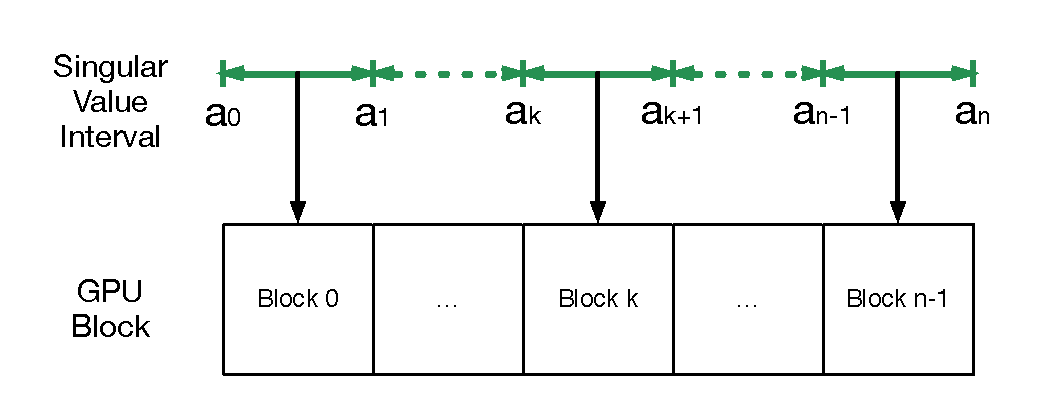
\includegraphics[width=0.4\textwidth]{length_interval}
  \label{fig:length_interval}
  }
  \\
  \vspace{-0.15in}
  \subfigure[Equal Number Division]
  {
  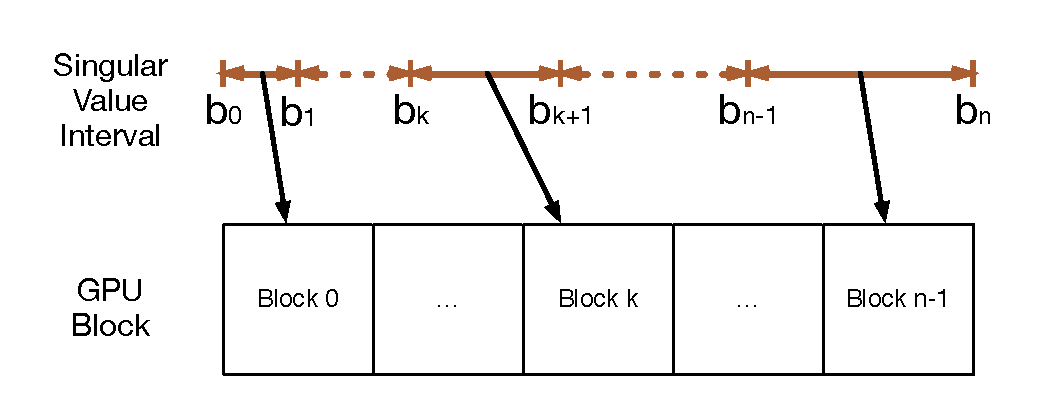
\includegraphics[width=0.4\textwidth]{number_interval}
  \label{fig:number_interval}
  }
\vspace{-0.1in}
\caption{Division Strategies for Partitioning Interval  $[a_0, a_n)$.} 
\vspace{-0.1in}
\end{figure}

The first (na\"{\i}ve) strategy is to divide the interval into chunks of equal length as shown in Fig.\ref{fig:length_interval}.
The whole interval $[a_0, a_n)$ is divided into $n$ subintervals with
the same length (i.e. same number of matrix elements). However, each
such subinterval might not contain the same number of singular values.
Mathematically, this strategy can be expressed as
$a_{k+1}-a_k = a_{k}-a_{k-1}$. However, $NegCount(b_{k+1})-NegCount(b_{k}) = NegCount(b_{k})-NegCount(b_{k-1})$ is not necessarily true. We call this strategy as {\it equal length division}.

Such ``equal length division'' strategy has issues in load balancing on 
parallel computing resources, as the number of singular values in each
subinterval is not uniform. As a result,
the SVD workload cannot be easily balanced on GPU's processing cores to achieve a satisfactory speedup because the optimal number of subintervals is dependent on multiple factors, such as the maximum number of threads, the number of threads in a GPU warp, and the size of matrix.
The maximum number of threads per block determines the minimum number
of subintervals that are assigned to corresponding GPU blocks.
In addition, the number of threads in a GPU warp assigned to a subinterval affects the GPU utilization level.

We have conducted experiments to understand the trade-offs between subinterval length and the GPU execution efficiency. 
Smaller subintervals will lead to a larger number of subintervals, which cause the GPU warp execution to be less efficient. 
For example, our experiments show that if $512$ subintervals are used, the efficiency of GPU warp execution ranges from only 12.38\% to 52.15\% when the matrix size increases from $1,000$ to $17,000$.
That is, only half of the threads in a warp work in parallel at most. This is because  (1)
 there are fewer singular values than the number of warps, leading the cores under-utilized; and 
(2) the warps are stalled due to memory accesses.
When the subinterval becomes larger, some block may get more singular values to calculate than its capability.
In order to achieve a higher speedup, we could try to find the optimal number of subintervals, or the number of blocks, based on experimental results. 
However, because of the uneven number of singular values within subintervals, the speedup for equal length division remains very limited, which motivates us to search for a better partition method.

Our novel strategy is to divide the whole interval by the number of singular values, as shown in Fig.\ref{fig:number_interval}. We call this approach {\it equal number division}. 
Specifically, we divide the interval $[b_0,b_n)$ into $n$ subintervals, each of which has the same number of singular values. 
However, the length of a subinterval is not necessarily equal to others.
The mathematical representation can be written as $NegCount(a_{k+1})-NegCount(a_{k})=NegCount(a_{k})-NegCount(a_{k-1})$ but $b_{k+1}-b_k = b_{k}-b_{k-1}$ does not necessarily hold anymore.
This equal number division significantly improves the load balancing on GPU cores, helping achieve a better speedup, as we show the performace evaluation in Figure \ref{fig:compare_value_kernel}.

The significant advantage for the equal number division strategy is that, more singular values can be calculated with the equal number division strategy than equal length division strategy.
Our experiment results show that equal number division outperforms length division strategy:
The warp execution efficiency in equal number division version can reach 92.97\%-96.13\%.

\subsection{Singular Vector Kernel} \label{sec_svector}
Since the singular vectors are two $n\times n$ dense matrices, as the matrix size increases, there is increasing pressure on memory storage because the size of the fast shared memory is limited in GPU architectures.
It is impracticable to move all the matrix entries to the shared memory when matrix size becomes extremely large.

Based on the twisted algorithm, the required memory size $M$ on GPU is determined by matrix size $n$ and the size of floating number $S$ in equation $M = 5 * S * n^2$, 5 is the number of arrays required for a pair of singular vectors.
For example, the maximum matrix size with $4$-bytes floating number values is about $10000$ for a GPU with $2$GB GPU memory. 
For matrices larger than that, we need to explore multiple GPUs to scale its performance as described in Section \ref{sec_mgpu}.

We initially implement the twisted algorithm with row-major matrix stored in the global memory
of a GPU system. 
We observe the heavy usage of global memory, which is
the slowest memory component on GPUs. 
Further analysis reveals that about 50\% of global memory transfers are read-after-write. Since it is a waste of time to read from global memory after writing to global memory,
we could improve the memory access performance by copying these values into the local memory and shared memory of the GPU.
The way to store matrix elements (column major or row major) is also critical as the memory accesses could be coalesced if the matrix elements
can be read and computed in large chunks. We present the results
of such optimizations in Section \ref{sec:results}.

\subsection{Solution to Big Matrices} \label{sec_huge}
In our design, the maximum number of singular values can be processed on a singular GPU is $m_b = subinterval\_size \times thread\_block\_size$,
while the maximum number of singular vectors are determined by $m_t = \sqrt{U / (5 * S)}$,
where $U$ is the memory size of GPU, 5 is mentioned above.
Usually, $m_b$ is much larger than $m_t$.
For Tesla K40c with 12GB memory, $m_t = 24K$, while $m_b = 262K$.
However, when the matrix size is larger than $m_t$, even larger than $m_b$,
the GPU kernels cannot obtain all singular values and vectors any more with a single GPU.
Therefore we derive a divide-and-conquer architecture to solve the huge matrix size as explained in this section.

When the size of a matrix is less than $m_b$ but larger than $m_t$,
we only need to divide the singular vectors into small sets, each of which can be processed by a single GPU.
However, if the matrix size is larger than $m_b$, we should divide both singular values and singular vectors into smaller partitions.
The singular value computations can be partitioned using $m_b$ directly, i.e., there are $l_b = \lfloor(n/m_b)\rfloor + 1$ partitions, each of which has $\lfloor(n/l_b)\rfloor$ singular values.

The division of singular vectors should take memory size into consideration.
The maximum number of partitions $l_t$ can be derived from Equation $l_t = \sqrt{U/(5 * n * 4)}$, 
where $n$ is matrix size.
Thus, there should be $\lfloor(n/l_t)\rfloor+1$ partitions with
$\lfloor(n/l_t)\rfloor$ singular vectors in each partition.

\subsection{Multiple GPUs on a server}\label{sec_mgpu}
We implement the multiple-GPU version with Pthread libraries on one server
to control data partition and assignment to GPUs.
Pthread is a nature choice for controlling multiple GPUs on a single server
because it uses shared memory architecture, dramatically reducing overheads
on data sharing. We also design an extensible interface between CPU and GPU,
 which is easy to scale to physical distributed GPUs, compared to CUDA asynchronization interface. In our design, each thread takes control of one GPU.

When matrix size becomes huge, the load balancing among multiple GPUs will be a problem for performance as shown in column 2 of Table \ref{tab:hugeResultTesla}.
To conquer this issue we also introduce a dynamic load-balancing method for a better speedup, where a GPU will take new tasks on unfinished subintervals as soon as it finishes its prior task.



\section{Experimental Results} \label{sec:results}
In this section, we evaluate the performance of our bisection and twisted algorithm and compare it with prior SVD implementations on CPUs and GPUs.
We implement the proposed BT algorithm on Tesla K40c with Kerpler architecture. 
Our implementation can also run on GeForce 750Ti with Maxwell architecture and Quandro with Fermi architecture.
In our implementations, we set the number of threads per GPU block as 512, which brings the better performance than other possible block sizes.
For the multi-GPU version of BT, we use 2 Tesla K40c that reside in the same server to scale up the size of matrices. 
It is worth noting that our multi-GPU version of BT algorithm can be extended to physically distributed GPUs, i.e., GPUs on different hosts connected via a high speed network. 
This part is however beyond the scope of this paper. 

\subsection{Comparison to Existing SVD Implementations}
We generate random bidiagonal matrices with double precision numbers in the range between 0 and 1.
It is reasonable because many application require to scale data to [0,1], and some singular values are always clustered when matrix size become large.
In order to achieve high confidence on the results, we generate 10 random matrices, and for each matrix, our SVD algorithm is executed 10 times on a GPU (or two GPUs).
The standard deviation of their execution time is very small, so we report the average execution time across the 100 runs as the performance results.

We compare our algorithm with CULA GPU library \cite{cula}, Intel MKL library \cite{mkl}, Sheetal's QR implementation on S1070 \cite{09IPDPSQR}, and Liu's DC implementation on M2070 \cite{13CFDC}.
We measure the performance of CULA on Tesla K40c, and that of Intel MKL on an 8-core 2.53GHz CPU.
Until now, CULA library only has a QR based routine called culaDbdsqr.
Intel MKL library has both DC routine DBDSDC and QR routine DBDSQR. We select a faster routine DBDSDC for a comparison.
For Sheetal's \cite{09IPDPSQR} and Liu's \cite{13CFDC} implementation, we use the experimental results presented in their paper. 

\begin{figure}[t]
\vspace{-0.1in}
\centering
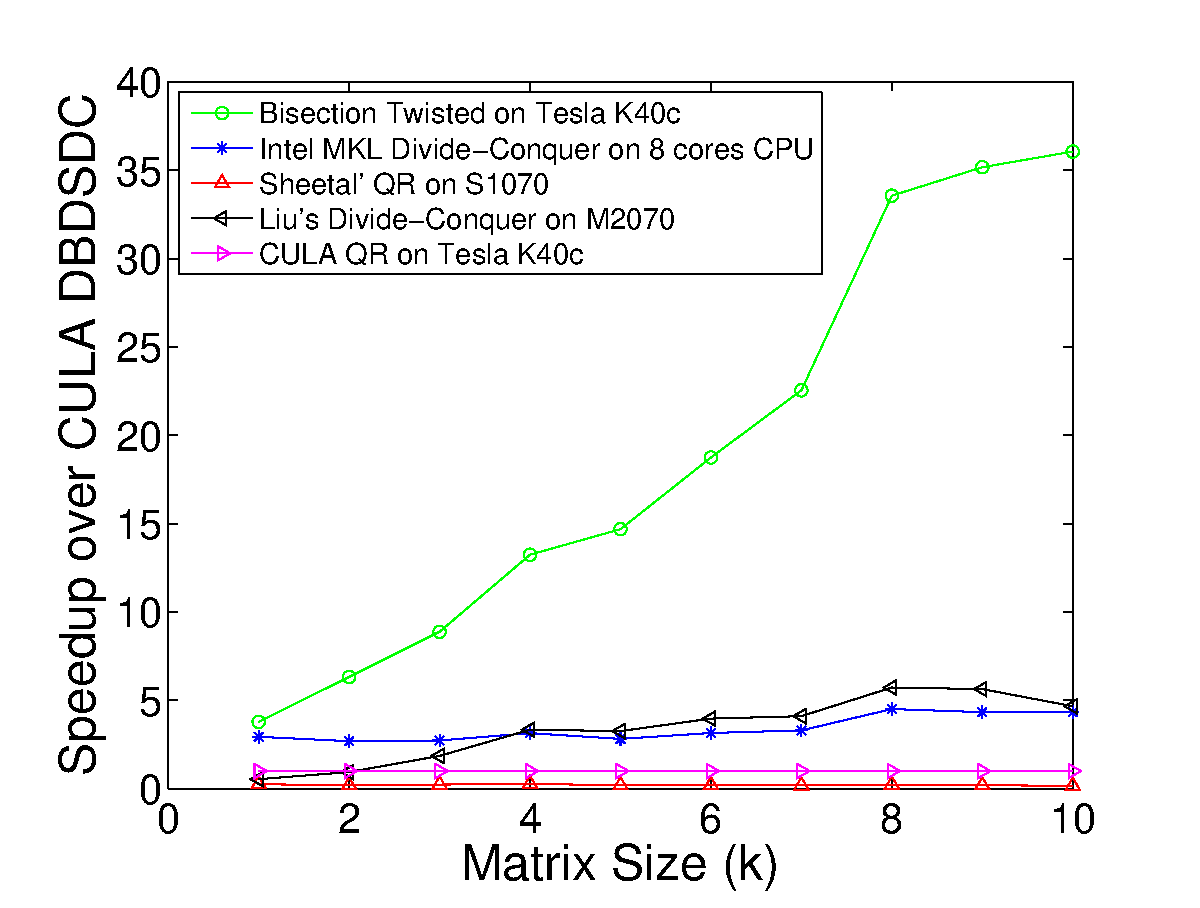
\includegraphics[width=0.4\textwidth]{svd_speedup}
\vspace{-0.1in}
\caption{Overall Performance Comparison}
\label{fig:svd_speedup}
\vspace{-0.2in}
\end{figure}
Figure \ref{fig:svd_speedup} shows the performance comparison of BT
implementation on Tesla K40c GPU to other existing libraries
and implementations.
The x-axis is the size of input matrix, and the y-axis is the speedup
using CULA QR routine DBDSQR as the baseline.
Our BT algorithm achieves a speedup of 3.8 to 36 over CULA culaDbdsqr routine,
while Intel MKL DBDSDC routine has a 2.9 to 4.3 speedup on a 8 core CPU and Liu's implementation achieves only 0.5 to 4.7 speedup over CULA library.
On the other hand, Sheetal's implementation is about 3 to 5.3 times slower than CULA library.

The performance of BT scales well when the matrix size becomes large.
Overall, we achieve a speedup of 1.3 to 8.3 over the Intel MKL
DC implementation on CPU, 4 to 7.2 over the Liu's
DC method on GPU, and 15 to 288 over the QR implementation in the work by Sheetal et al.
Now let us take a look at each of the algorithms from the perspective of matrix size, Sheetal's QR implementation and Liu's DC implementation do not work at all when the dimensions of matrices are larger than 14K by 14K on their GPU with memory size of 16GB and 6GB, respectively. In contrast, in our implementation, the matrix size could reach 1 million by 1 million as shown in Table \ref{tab:hugeResultTesla}.

%\subsection{Performance Comparison on Different GPUs}
%\subsubsection{Singular Value Computation}
%\begin{figure}[hbpt]
%\vspace{-0.2in}
%\centering
%  \subfigure[Execution time]
%  {
%    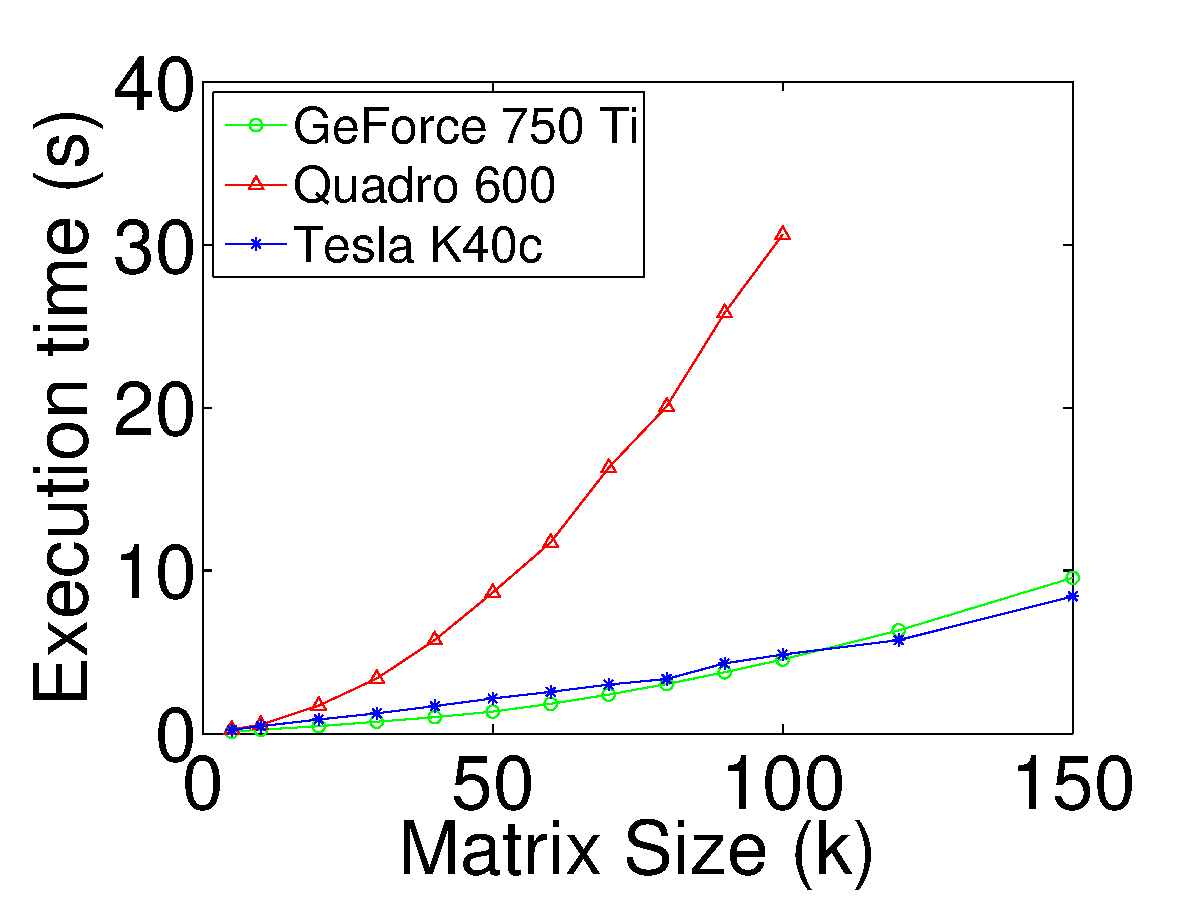
\includegraphics[width=0.25\textwidth,height=1in]{svd_val_gpus}
%    \label{fig:svd_val}
%  }
%  \\
%\vspace{-0.1in}
%  \subfigure[Profiling Data]
%  {
%    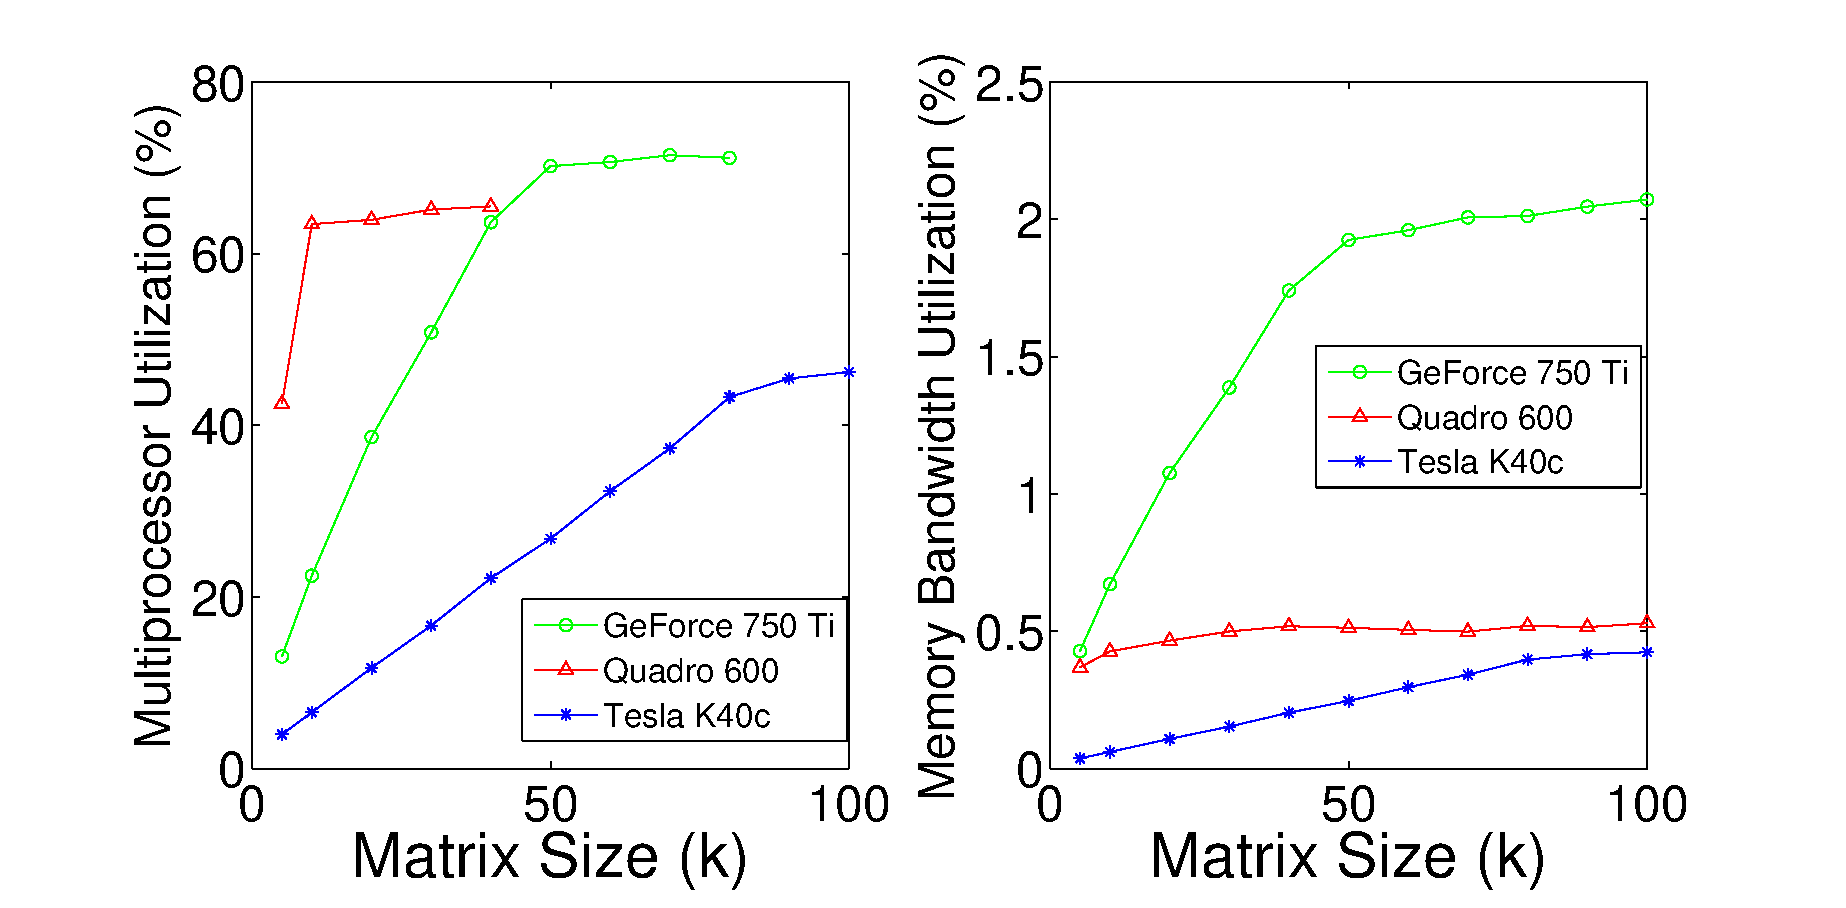
\includegraphics[width=0.45\textwidth,height=1in]{svd_val_gpus_prof}
%    \label{fig:svd_val_prof}
%  }
%\vspace{-0.1in}
%  \caption{Singular Value Kernel on Different GPUs}
%  \label{fig:svdval}
%\vspace{-0.15in}
%\end{figure}
%
%Figure \ref{fig:svd_val} shows the execution time of calculating singular values with our ``equal number division'' design on different GPUs with single-precision floating point.
%Quadro has the worst performance, while performance of GeForce and Tesla are close to each other.
%In particular, When the matrix size is less than $100K$, GeForce is slightly better. Otherwise, Tesla is better. 
%
%To understand the reasons
%of such performance differences, we conduct a series of profiling experiments.
%Figure \ref{fig:svd_val_prof} shows the thread activity and memory bandwidth utilizations of singular value kernels on different GPUs, for matrices of size up to 
%100K (unfortunately we are unable to get profiling data for matrices of larger size due to the overflow of profiling counters). 
%The figure shows that the thread utilization reaches 70\% on Quadro and GeForce, and 50\% on Tesla. 
%But the memory bandwidth utilization is only 0.1\%-2\%.
%The main reason is that singular value computations rely on the fast shared memory
%of GPUs due to its low memory requirements. That is, finding the singular
%values is rather CPU-bound than memory-bound. 
%As a result, the performance is determined largely by the number of CUDA cores and the ratio of thread activity on a GPU.
%
%\subsubsection{Singular Vector Computation}
%Figure \ref{fig:svd_vec} shows the execution time of singular vector kernel on different GPUs. 
%It is easily seen that GeForce is about 8 times faster than
%Quadro. This is because GeForce has a much higher memory bandwidth
%than Quadro.
%In addition, the device memory read/write transactions of GeForce are only 1/6 and 1/4 of those of Quadro, respectively.
%The performance on Tesla is slightly better than that on GeForce.
%Tesla has nearly the same device memory read transactions as GeForce does, while 3 times more write transactions than GeForce.
%%Yet Tesla is still the winner of the three because of its extremely high bandwidth as listed in Table~\ref{tab:spec}.
%
%\begin{figure}[hbpt]
%\vspace{-0.1in}
%\centering
%  \subfigure[Execution time]
%  {
%    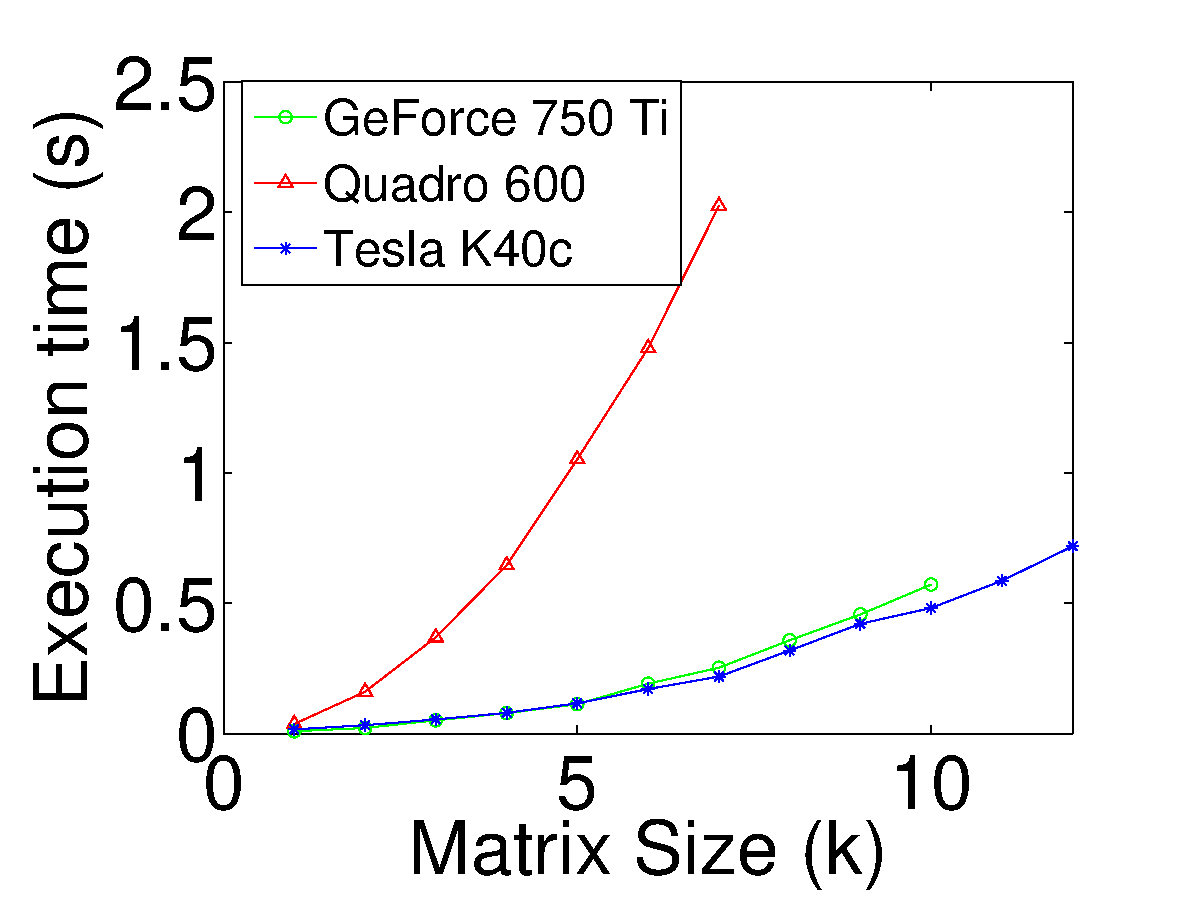
\includegraphics[width=0.3\textwidth,height=1in]{svd_vec_gpus}
%    \label{fig:svd_vec}
%  }
%\\
%\vspace{-0.1in}
%  \subfigure[Profiling Data]
%  {
%    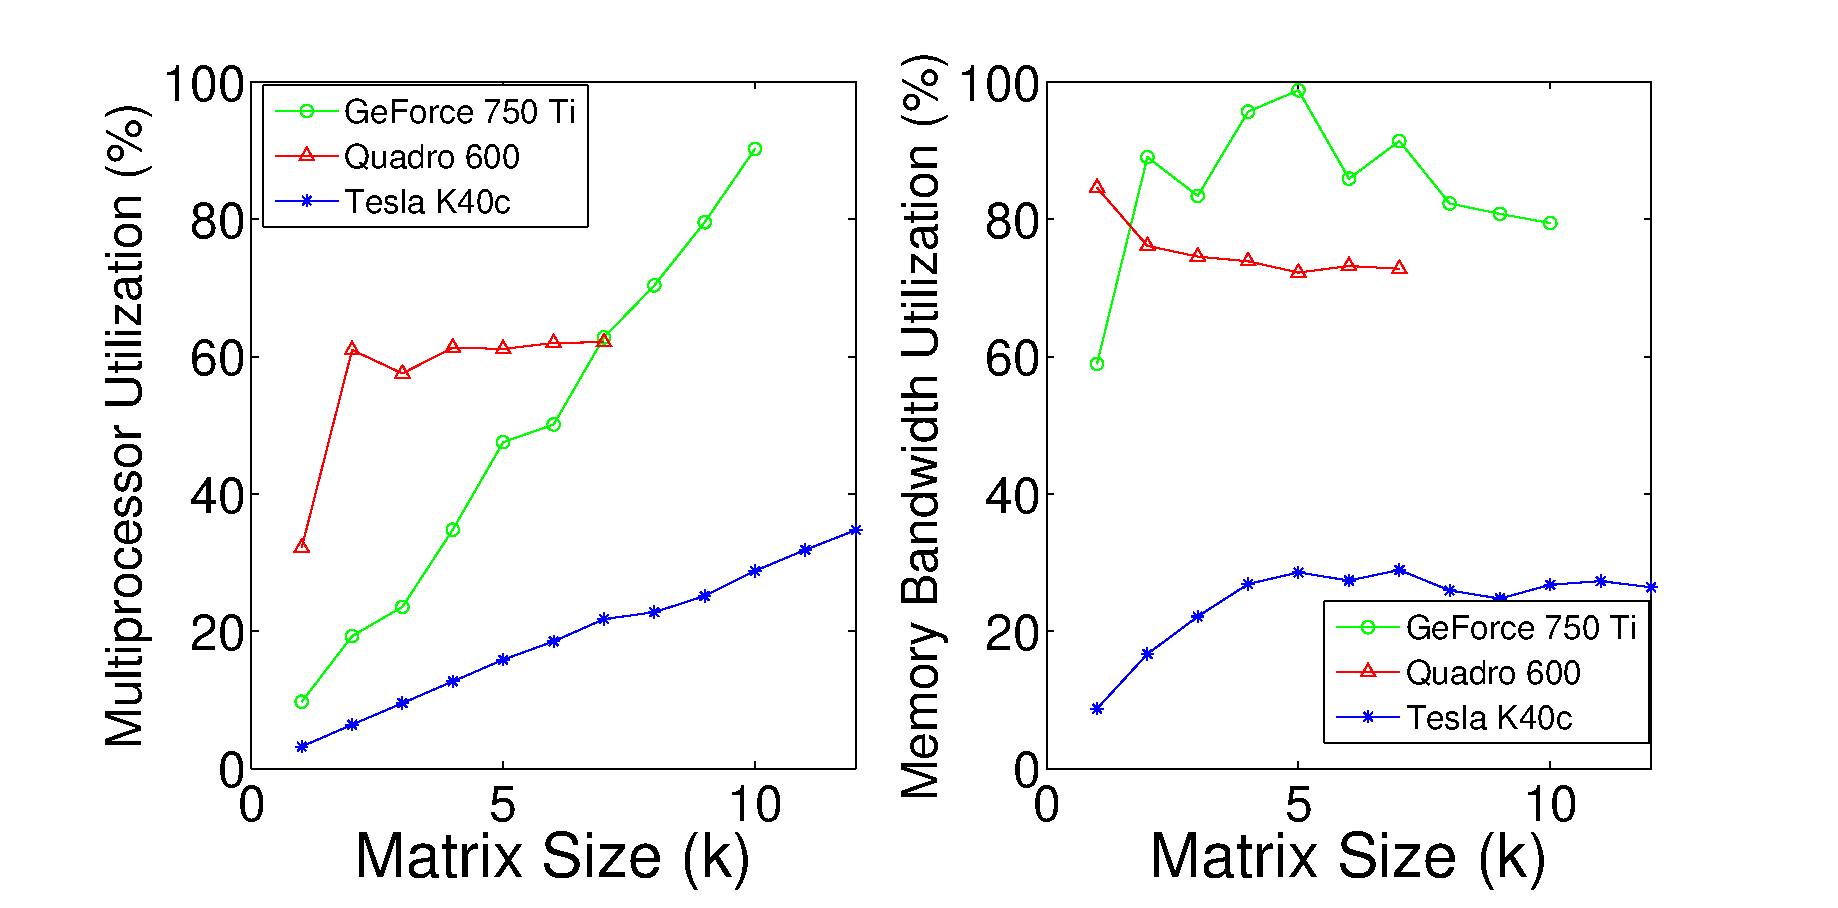
\includegraphics[width=0.45\textwidth,height=1in]{svd_vec_gpus_prof}
%    \label{fig:svd_vec_prof}
%  }
%\vspace{-0.1in}
%  \caption{Singular Vector Kernel on Different GPUs}
%  \label{fig:svdvec}
%\vspace{-0.15in}
%\end{figure}
%
%Figure \ref{fig:svd_vec_prof} shows thread and memory bandwidth utilizations of singular vector design on different GPUs. 
%We can see from the figure that Quadro and GeForce reach a high memory utilization (80\%-99\%), while the memory utilization of Tesla is around 30\%. 
%We also observe that when the matrix size is larger than 2K, the thread utilization keeps stable on Quadro. 
%This is because the ratio of stall caused by memory is 70\%, implying that there are a lot of threads waiting on data transfer.

\subsection{Experiments with Big Matrices}
Table \ref{tab:hugeResultTesla} shows the performance of very large matrix with double-precision floating-point numbers on a single Tesla and two Tesla GPUs on a server. For two Telsa GPUs, we compared static workload allocation (50\%/50\%) and dynamic allocation where each GPU is tracked constantly by the host CPU and assigned new workload as soon as it finishes the current kernel. 
When matrix size reaches 1 million by 1 million our BT algorithm reaches the results in 54801 seconds with a single Telsa, and 35607 seconds with two Telsa GPUs. This is a 1.54X speedup.
\begin{table}[t]
\vspace{-0.1in}
\caption{Performance of Huge Size Matrix with double floating-point on Tesla}
\vspace{-0.1in}
\centering
\begin{tabular}{|c|c|c|c|}
\hline
Matrix Size &  Tesla  & Static (2-GPU) & Dynamic (2-GPU) \\ \hline
 50K*50K    &    71s  &   50s /  45s &  44s / 44s \\ \hline
 100K*100K  &   341s  &  217s / 189s &  210s / 202s \\ \hline
 150K*150K  &   864s  &  524s / 467s &  498s / 507s \\ \hline
 200K*200K  &  1407s  &  955s / 827s &  849s / 858s \\ \hline
 300K*300K  &  3490s  & 2234s / 1906s & 2123s / 2110s\\ \hline
 400K*400K  &  6559s  & 4110s / 3709s & 3853s / 3871s\\ \hline
 500K*500K  & 12282s  & 7371s / 6916s  & 7148s / 7129s\\ \hline
 800K*800K  & 40311s  & 22454s / 21627s &  22046s / 22026s   \\ \hline
 1000K*1000K & 54801s  & 36119s / 35071s   &  35587s / 35607s \\ \hline
\end{tabular}
\label{tab:hugeResultTesla}
\vspace{-0.1in}
\end{table}


\subsection{Profiling Analysis of GPU Kernels}
\subsubsection{Comparison of Two Different Singular Value Designs}
We compare the execution time on two different singular value kernels:
``equal length division'' versus ``equal number division''. Each
method has two phases: (1) divide the interval into subintervals and
(2) calculate singular values in each subinterval.
\begin{figure}[htbp]
\vspace{-0.1in}
\centering
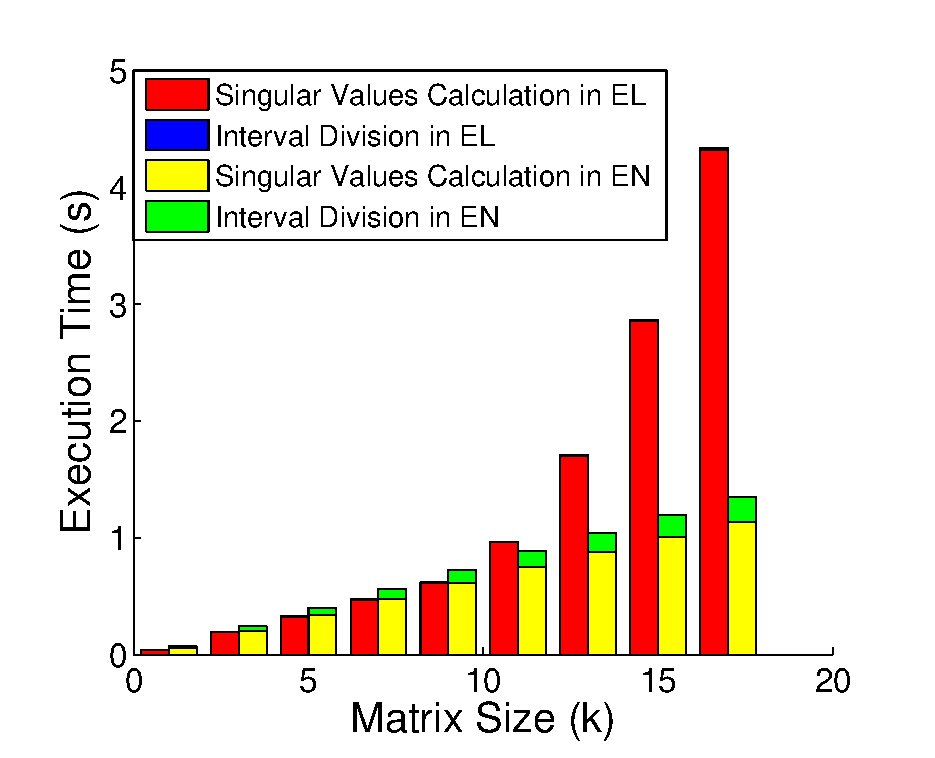
\includegraphics[width=0.4\textwidth]{compare_value_kernel}
\vspace{-0.1in}
\caption{Comparison of Equal Length Division and Equal Number Division.}
\label{fig:compare_value_kernel}
\vspace{-0.1in}
\end{figure}
Figure \ref{fig:compare_value_kernel} shows the detailed execution time breakdown for each phase of both methods (``Interval Division'' time for ``equal-length division'' is negligible) on Tesla K40c.
From the figure, we can see that when the matrix size is less than 9K, the equal length division version runs a little faster than equal number division version.
However, when the matrix size exceeds 9K, the execution time of the equal length division version increases dramatically, while the execution time of equal number division version still rises linearly.
And in this case, 
even though the time to divide the interval is noticeably
large, the balanced number of singular values in a subinterval
still yields much better performance.
Thus, the equal number division version is obviously the winner when the matrix size becomes larger than 9K.

\begin{figure}[hbpt]
\centering
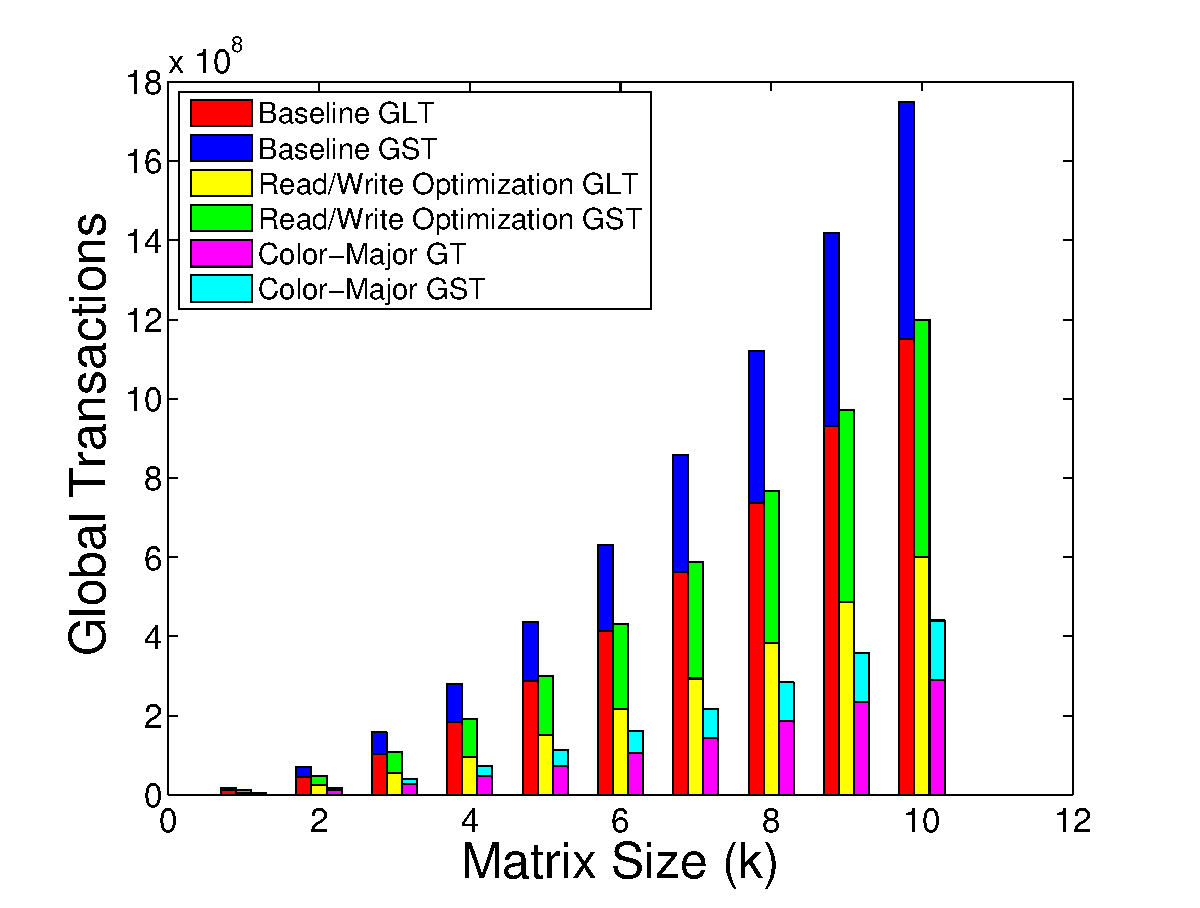
\includegraphics[width=0.4\textwidth]{transaction}
\vspace{-0.1in}
\caption{Memory Transactions on Singular Vector Design}
\label{fig:transaction}
\vspace{-0.2in}
\end{figure}
\subsubsection{Memory Access Optimization}
We evaluate the memory optimization techniques on improving the performance
of singular vector calculation. As depicted in Figure \ref{fig:transaction},
in the baseline design,
Global memory Load Transactions (GLT) are about twice of the Global memory Store Transactions (GST) on the global memory.
As there are 50\% of global memory transfers are read-after-write, we improve the memory access performance by copying these values into the local memory and shared memory of the GPU. As a result, the GLT are reduced by 50\% compared to the baseline, while the GST remains the same, labeled as ``Read/Write Optimization'' in Figure \ref{fig:transaction}. The speedup on singular vector calculation reaches to 1.2X compared to the baseline.
Changing the matrix arrangement from row-major to column-major in the global memory 
reduces GLT and GST by 50\% and 25\%, respectively, compared to ``Read/Write optimization''. 
This is because column-major matrix have coalesced global memory accesses, which saves hundreds of transactions per thread. The speedup rises up to 4.5X compared to the baseline.

\subsection{Accuracy Analysis}
\subsubsection{Tolerance in Bisection Algorithm}
Bisection algorithm is an approximate algorithm to calculate the singular values, we should evaluate the effect of different error tolerance.
The error tolerance $err$ means that the error between the singular values of our algorithm and the actual singular values are less than $err$.
It determines the accuracy of singular value and therefore the orthogonality of singular vectors.
%As we know, the more accuracy of singular values are, the more execution time should be spent.
However, it is important to know the incremental execution time to determine which error tolerance is suitable for different applications.
%We test our algorithm on different error tolerance.
The error tolerance is between $10^{-5}$ to $10^{-16}$ with tenfolder decreasing.

\begin{figure}[htbp]
\vspace{-0.1in}
\centering
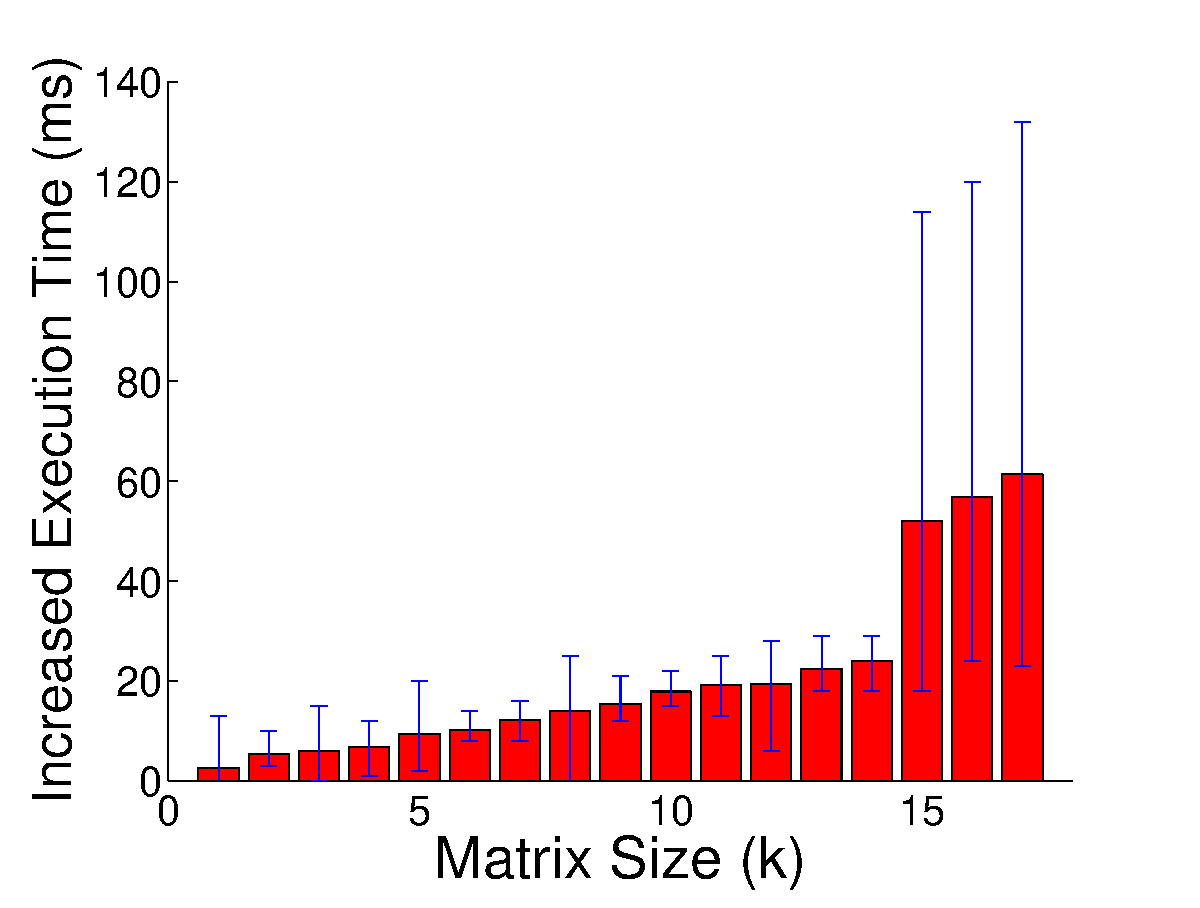
\includegraphics[width=0.4\textwidth]{tolerance}
\vspace{-0.1in}
\caption{Average Extra Time When Accuracy Increase}
\label{fig:tolerance}
\vspace{-0.1in}
\end{figure}
Figure \ref{fig:tolerance} shows the average increased execution time when the accuracy of singular values goes up a higher level.
In other word, it shows the average increased execution time when the error tolerance becomes smaller from $10^{-x}$ to $10^{-(x+1)}, (x=5,\cdots,15)$.
The additional execution time is less than $20 ms$ when matrix size is smaller than 12000, and $40 ms$ when matrix size is larger than 15000.
In either case, the increased time is negligible compared to the overall exeuction time.

\begin{figure}[hbpt]
\vspace{-0.1in}
\centering
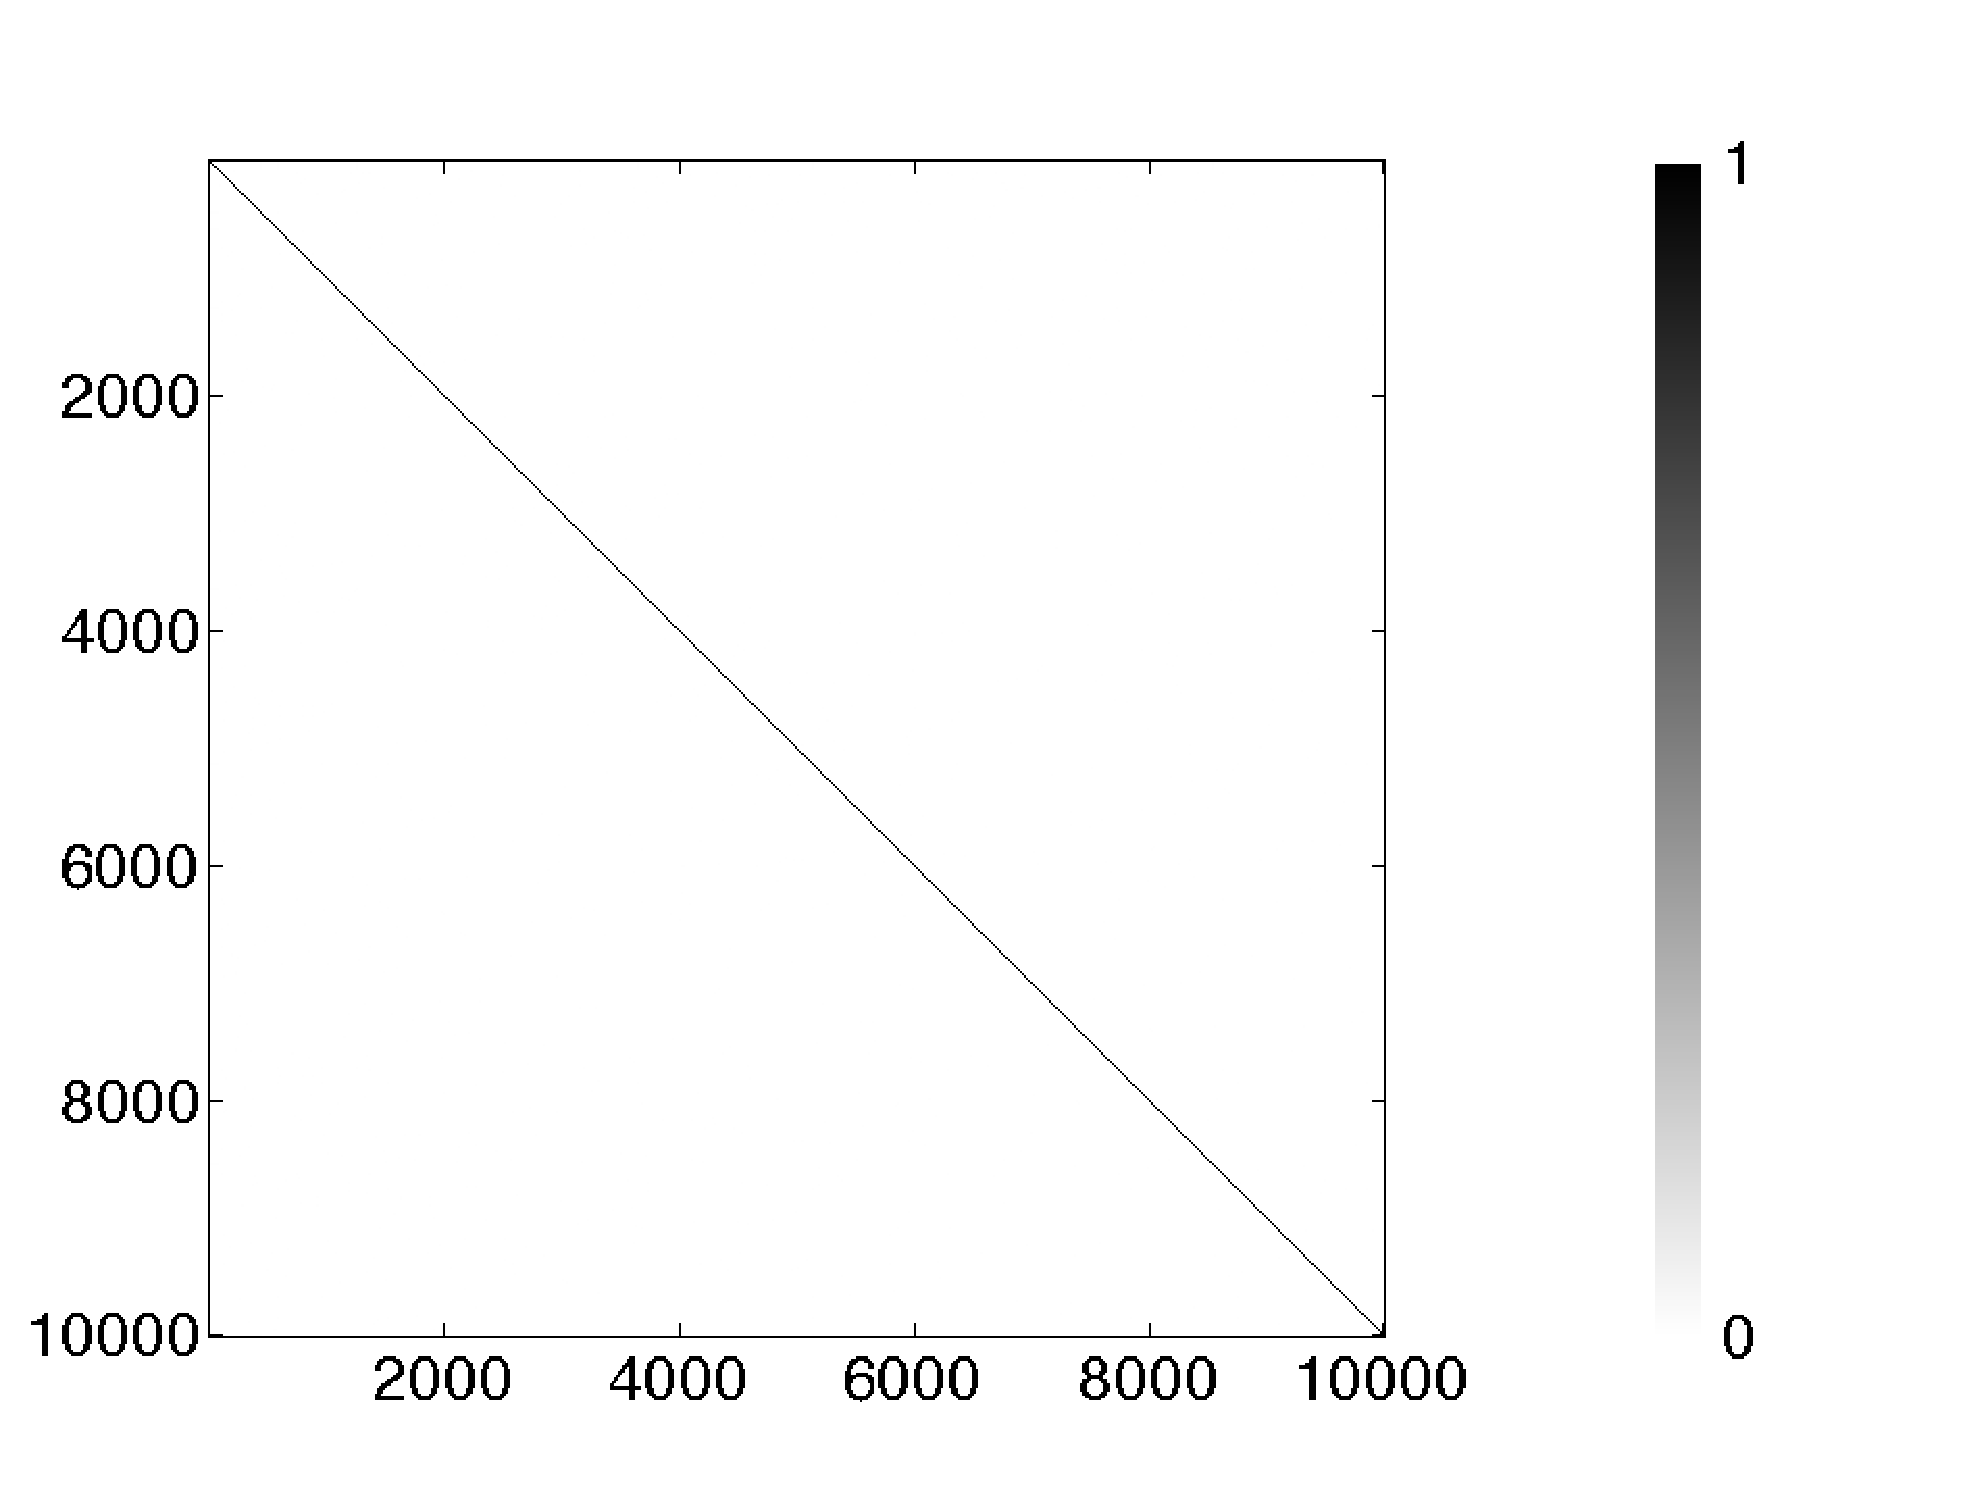
\includegraphics[width=0.4\textwidth]{orthogonal}
\vspace{-0.1in}
\caption{Orthogonality of Singular Vector}
\label{fig:ortho_img}
\vspace{-0.1in}
\end{figure}
\subsubsection{Orthogonality of Singular Vector}
Figure \ref{fig:ortho_img} shows the image of multiplication of singular vectors when matrix size is 10000.
The element in white areas are close to 0s, and the element in black diagonal are 1s.
It shows our implementation has good orthogonality.

%Figure \ref{fig:ortho_err} shows the error distribution of orthogonality of a 10K$\times$10K matrix. We define the orthogonal error is the element in $U\times U^T - I$. The maximum orthogonal error is less than 0.02.


\section{Related Work} \label{sec:related}
General purpose GPUs become important processing engines for computationally intensive workloads due to their highly parallel computing architectures.
CUBLAS provides many solutions for low-level linear algebra operations supported by Nvidia \cite{cublas}. 
CULA consists of commercial hybrid GPU accelerated linear algebra routines \cite{cula}.
MAGMA aims to achieve high performance and portability across a wide range of multi-core architectures and hybrid systems respectively\cite{magma}.

The first SVD algorithm with CUDA programming is implemented by Sheetal et al.\cite{09IPDPSQR}. With parallelized QR iteration algorithm using CUBLAS library on GPU, they achieved a speedup of up to 8 over the Intel MKL QR implementation.
Liu et al. use a divide-and-conquer approach to solve SVD on a heterogeneous CPU-GPU system \cite{13CFDC}.
It is almost 7 times faster than CULA QR algorithm executing on the same device M2070, and up to 33 times faster than LAPACK.
Vedran\cite{14arxivjacobi} presents a hierarchically blocked one-sided Jacobi algorithm for the singular value decomposition on both single and multiple GPU architectures. Even with full optimizations and a high speedup compared to the same algorithm on CPU, the execution time is still more than that of QR implementation.

Drineas et al. \cite{99clustering} provide a clustered SVD algorithm for large matrices. The algorithm divides a set of $n$ points into $k$ clusters, where $k$ is much less than $n$ on CPU.
It is an approximation algorithm to obtain only one subset of singular values
and vectors. Our BT algorithm can compute the complete SVD, thus is not
directly compared with \cite{99clustering}. 



\section{Conclusion} \label{sec:conclusion}
We present a novel algorithm for computing singular values and vectors called bisection and twisted (BT) algorithm, 
which is implemented on both single GPUs and a multi-GPU platform.
The experimental results show that BT outperforms a number of existing
work on SVD acceleration. %Additionally, BT's scalability is excellent:
One of the major advantages for BT algorithm is its scalability:
we are the first to perform SVD on a matrix of 1 million by 1 million,
using only two GPUs. In the near future, we plan to extend our multi-GPU version of BT
with network middleware such as MPI so that BT algorithm can be further 
extended to distributed GPUs.
%scaled with GPU clusters.



% An example of a floating figure using the graphicx package.
% Note that \label must occur AFTER (or within) \caption.
% For figures, \caption should occur after the \includegraphics.
% Note that IEEEtran v1.7 and later has special internal code that
% is designed to preserve the operation of \label within \caption
% even when the captionsoff option is in effect. However, because
% of issues like this, it may be the safest practice to put all your
% \label just after \caption rather than within \caption{}.
%
% Reminder: the "draftcls" or "draftclsnofoot", not "draft", class
% option should be used if it is desired that the figures are to be
% displayed while in draft mode.
%
%\begin{figure}[!t]
%\centering
%\includegraphics[width=2.5in]{myfigure}
% where an .eps filename suffix will be assumed under latex, 
% and a .pdf suffix will be assumed for pdflatex; or what has been declared
% via \DeclareGraphicsExtensions.
%\caption{Simulation Results}
%\label{fig_sim}
%\end{figure}

% Note that IEEE typically puts floats only at the top, even when this
% results in a large percentage of a column being occupied by floats.


% An example of a double column floating figure using two subfigures.
% (The subfig.sty package must be loaded for this to work.)
% The subfigure \label commands are set within each subfloat command, the
% \label for the overall figure must come after \caption.
% \hfil must be used as a separator to get equal spacing.
% The subfigure.sty package works much the same way, except \subfigure is
% used instead of \subfloat.
%
%\begin{figure*}[!t]
%\centerline{\subfloat[Case I]\includegraphics[width=2.5in]{subfigcase1}%
%\label{fig_first_case}}
%\hfil
%\subfloat[Case II]{\includegraphics[width=2.5in]{subfigcase2}%
%\label{fig_second_case}}}
%\caption{Simulation results}
%\label{fig_sim}
%\end{figure*}
%
% Note that often IEEE papers with subfigures do not employ subfigure
% captions (using the optional argument to \subfloat), but instead will
% reference/describe all of them (a), (b), etc., within the main caption.


% An example of a floating table. Note that, for IEEE style tables, the 
% \caption command should come BEFORE the table. Table text will default to
% \footnotesize as IEEE normally uses this smaller font for tables.
% The \label must come after \caption as always.
%
%\begin{table}[!t]
%% increase table row spacing, adjust to taste
%\renewcommand{\arraystretch}{1.3}
% if using array.sty, it might be a good idea to tweak the value of
% \extrarowheight as needed to properly center the text within the cells
%\caption{An Example of a Table}
%\label{table_example}
%\centering
%% Some packages, such as MDW tools, offer better commands for making tables
%% than the plain LaTeX2e tabular which is used here.
%\begin{tabular}{|c||c|}
%\hline
%One & Two\\
%\hline
%Three & Four\\
%\hline
%\end{tabular}
%\end{table}


% Note that IEEE does not put floats in the very first column - or typically
% anywhere on the first page for that matter. Also, in-text middle ("here")
% positioning is not used. Most IEEE journals/conferences use top floats
% exclusively. Note that, LaTeX2e, unlike IEEE journals/conferences, places
% footnotes above bottom floats. This can be corrected via the \fnbelowfloat
% command of the stfloats package.




% conference papers do not normally have an appendix


% use section* for acknowledgement
\section*{Acknowledgment}

This work is support in
part by the National Science Foundation under grant number
ACI-1440737 and grant number ACI-1450996. 

% trigger a \newpage just before the given reference
% number - used to balance the columns on the last page
% adjust value as needed - may need to be readjusted if
% the document is modified later
%\IEEEtriggeratref{8}
% The "triggered" command can be changed if desired:
%\IEEEtriggercmd{\enlargethispage{-5in}}

% references section

% can use a bibliography generated by BibTeX as a .bbl file
% BibTeX documentation can be easily obtained at:
% http://www.ctan.org/tex-archive/biblio/bibtex/contrib/doc/
% The IEEEtran BibTeX style support page is at:
% http://www.michaelshell.org/tex/ieeetran/bibtex/
%\bibliographystyle{IEEEtran}
% argument is your BibTeX string definitions and bibliography database(s)
%\bibliography{IEEEabrv,../bib/paper}
%
% <OR> manually copy in the resultant .bbl file
% set second argument of \begin to the number of references
% (used to reserve space for the reference number labels box)

\bibliographystyle{abbrv}
\bibliography{ref}



% that's all folks
\end{document}


